\section{Diodo 1N4007: caratteristica volt-amperometrica}

\begin{wrapfigure}[22]{r}[0pt]{130mm}
	\caption{ciao}
	\label{fig:diodo}
	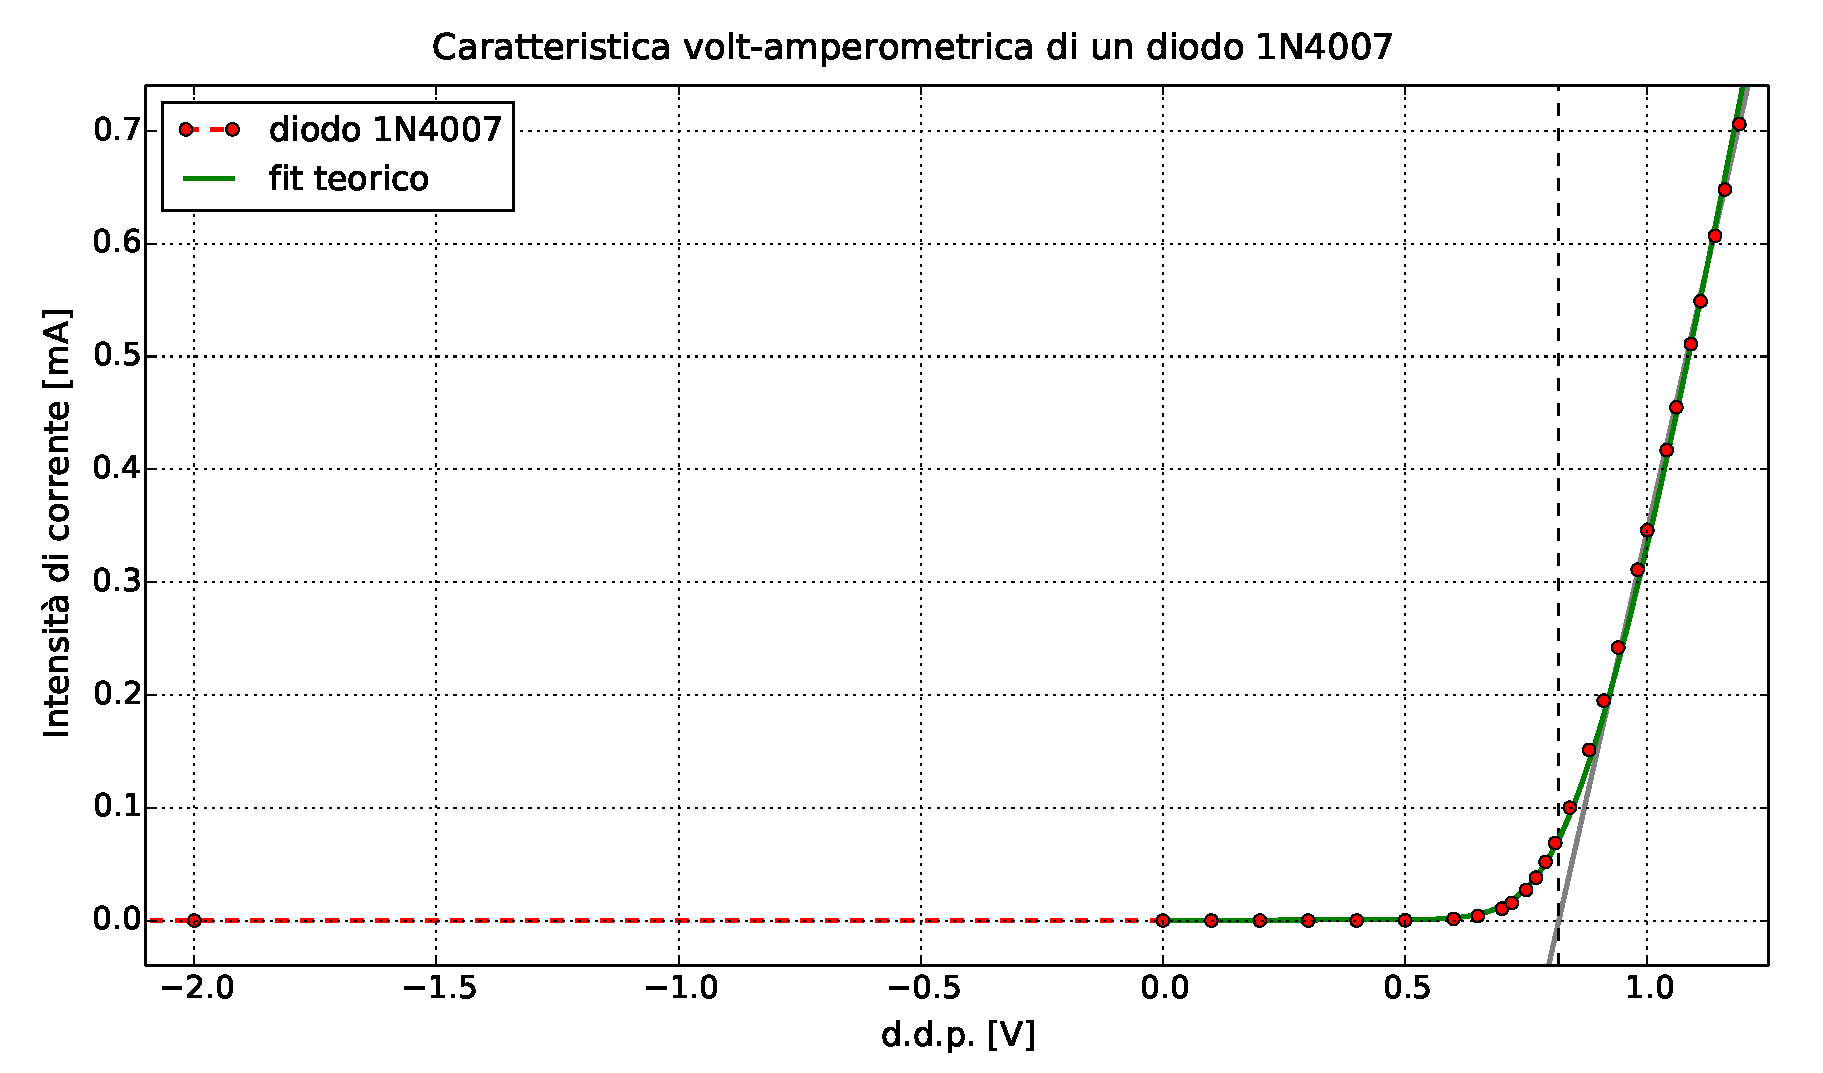
\includegraphics[width=0.75\textwidth]{diodo.pdf}
\end{wrapfigure}

Per studiare la caratteristica volt-amperometrica del diodo abbiamo dovuto separare l'analisi in due fasi distinte: una prima fase in cui abbiamo analizzato il comportamento del diodo polarizzato in diretta e una seconda fase in cui ne abbiamo analizzato il comportamento in inversa.
Utilizzando la breadboard come support,o abbiamo creato un circuito composto dal genertore di tensione continua (max $\pm \SI{25}{\volt}$), il diodo e il multimetro digitale in modalità amperometro. Aumentando progressivamente la tensione, abbiamo letto sull'amperometro i valori della corrente che attraversava il circuito.
Facendo attenzione che la corrente non superasse il valore di \SI{700}{\milli\ampere} abbiamo quindi popolato l'asse positivo del grafico. In seguito abbiamo girato il diodo in modo che fosse alimentato in inversa e abbiamo popolato anche l'asse negativo del grafico, ottenendo la caratteristica volt-amperometrica completa del diodo. Il risultato è esposto in Figura \ref{fig:diodo}.
\\
\\
Dal grafico osserviamo che i dati ricavati seguono la legge teorica, la cui formula è:
\begin{equation}
I_{D} \, = \, I_{S} \left( e^{\frac{q V_d}{nKT}} -1 \right)
\label{eq:diode}
\end{equation}

\section{Cella solare: caratteristica volt-amperometrica}

Abbiamo studiato la caratteristica volt-amperomentrica di una cella solare lavorando allo stesso modo di come abbiamo fatto per il diodo.
%\subsection{cella solare al buio}
La prima analisi sul comportamento della cella è stata svolta tenendo la cella solare al buio nella sua scatola, mentre una seconda analisi è stata completata con la cella solare sottoposta alla radiazione di una lampada da tavolo, facendo attenzione che quest'ultima non variasse significativamente di intensità.
Durante questa parte dell'esperienza abbiamo avuto cura che la corrente massima da cui era attraversata la cella non superasse i \SI{100}{\milli\ampere}. I dati ottenuti sono graficati in Figura \ref{fig:cella}.

\begin{figure}[h]
\center
	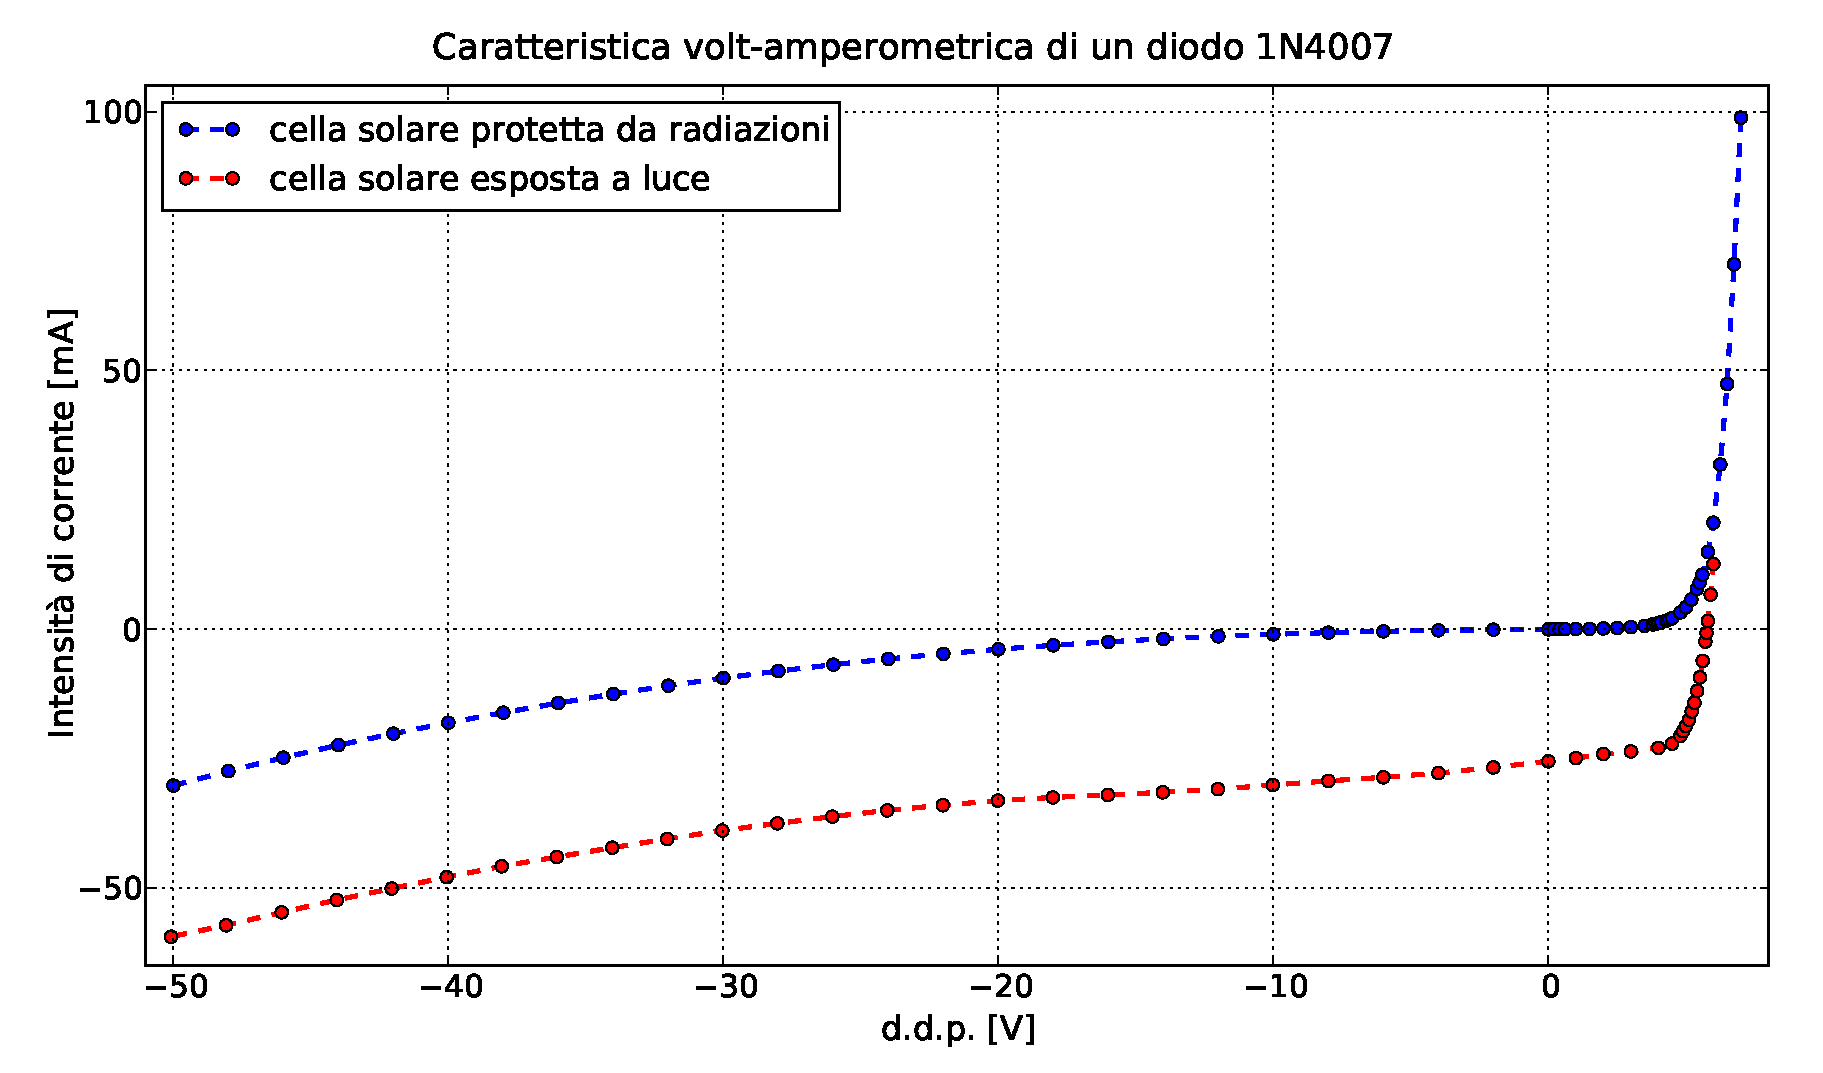
\includegraphics[width=0.75\textwidth]{cella.pdf}
	\caption{ciao}
	\label{fig:cella}
\end{figure}


\begin{equation}
FF \, = \, \frac{I_{@P_{max}} \,\, V_{@P_{max}}}{I_{sc} \,\, V_{oc}}
\label{eq:FF}
\end{equation}

%\subsection{cella solare alla luce}


\section{Ponte di Graetz}

Un ponte costituito da diodi può essere utilizzato come elemento raddrizzatore di un segnale. Riportiamo in Fig.() lo schema del ponte di Graetz da noi utilizzato. Tale ponte permette di raddrizzare un segnale in entrata, ovvero di fare in modo che un'uscita del ponte sia sempre più positiva dell'altra. Poichè i diodi hanno una caduta di tensione in diretta e una tensione di soglia, il segnale raddrizzato non potrà superare in tensione massima quella del segnale in entrata e inoltre il segnale raddrizzato sarà pari a 0 se la tensione in entrata non supera il valore di soglia.

Poichè l'oscilloscopio è collegato a massa, non è possibile visualizzare a schermo contemporaneamente sia segnale in input che segnale in uscita dal ponte. Si è dunque utilizzata l'impostazione $Permanenza$, la quale fa rimanere sullo schermo l'ombra dei segnali visualizzati. \'E stato così possibile osservare sull'oscilloscopio entrambi i segnali. Ricordiamo che la resistenza da noi utilizzata come carico aveva un valore di $R_L=9998 \pm 1$.

Nel seguente grafico sono riportati i segnali da noi visualizzati.

**grafico**


Avendo utilizzato un segnale sinusoidale in input vediamo che per valori di $V \approx 0$ i diodi non sono in conduzione e dunque la d.d.p in output risulta nulla. \'E importante osservare come la frequenza del segnale in uscita sia raddoppiata. Infatti per ogni periodo della funzione sinusoidale fornita dal generatore abbiamo due periodi della funzione in uscita. Ora che abbiamo ottenuto un segnale raddrizzato, sarebbe interessante trovare un modo per ottenere un segnale di tensione DC. Ciò è possibile utilizzando un condensatore da mettere in parallelo al carico in uscita dal ponte di diodi. Lo schema è riportato in Fig.(). La capacità gioca un ruolo fondamentale in quanto caricandosi e scaricandosi manda in interdizione i diodi del ponte, causando una stabilizzazione del segnale su un valore medio che dipende dalla capacità stessa. Per valori di capacità $C\neq 0$ il valore medio di tensione in uscita dal ponte si sposta su valori più alti. Inoltre, la forma d'onda in uscita risulta tanto più simile ad una scarica/carica di un condensatore quanto più alto è il valore di capacità. Il segnale che si vede a schermo risulta dunque simile alla sovrapposizione di un segnale oscillante con uno continuo. Tale fenomeno viene comunemente chiamato $Ripple$. Si definisce il fattore di ripple come: $r_f= \frac{V_{AC}}{V_{DC}}$, dove $V_{AC}$ è la differenza picco-picco del segnale mentre $V_{DC}$ la sua media. Per calcolare $V_{DC}$ abbiamo utilizzato la funzione integrata dell'oscilloscopio che esegue una media integrale. Riportiamo in tabella i dati da noi ottenuti:

\begin{SCtable}[20][h]
\centering
\caption{Dati da noi registrati con relativi errori.}
{\renewcommand{\arraystretch}{1.6}%
\begin{tabular}{c|c|c|c|c}
Capacità [$\si{\nano\farad}$] & Frequenza [$\si{\hertz}$] & $V_{AC}$ ripple [$\si{\volt}$] & $V_{DC}$ [$\si{\volt}$] & $r_f$ \\      \hline
$401 \pm 2$ &$100.1 \pm 0.1 $& $6.93 \pm 0.01$ & $6.87 \pm 0.01$ & $1.01 \pm 0.02$\\
$799 \pm 5$ &$100.2 \pm 0.1$& $5.28 \pm 0.01$ & $7.57 \pm 0.01$ & $0.70 \pm 0.02$\\
$1196 \pm 5$ &$100.1 \pm 0.1$& $4.42 \pm 0.01$ & $8.06 \pm 0.01$ & $0.55 \pm 0.02$\\
$4959 \pm 3$ &$100.3 \pm 0.1$& $1.45 \pm 0.01$ & $9.25 \pm 0.01$& $0.16 \pm 0.02$\\
\end{tabular}}
\end{SCtable}

Come ci aspettavamo, aumentando la capacità aumenta anche il valore $V_{DC}$. Inoltre vi è anche un sensibile smorzamento delle fluttuazioni del segnale attorno a tale valor medio. Per ottenere una tensione continua stabile è dunque preferibile utilizzare una capacità più grande possibile, così da minimizzare in fattore $r_f$.

Riportiamo infine un grafico dei segnali a schermo per ottenuti per la capacità $C=stocazzo$. Come si può vedere, la forma d'onda in uscita non è più simile al valore assoluto del segnale in ingresso ma ad una serie di scariche/cariche di un condensatore.



 